
\documentclass{standalone}
\usepackage[utf8]{inputenc}
\usepackage{hyphsubst}
%\HyphSubstIfExists{ngerman-x-latest}{
%  \HyphSubstLet{ngerman}{ngerman-x-latest}}{}
%\HyphSubstIfExists{german-x-latest}{
%  \HyphSubstLet{german}{german-x-latest}}{}
\usepackage{zi4}
\usepackage{amsmath} %for matrices
\usepackage{amssymb} %for element of N / R etc
\usepackage{amsthm} % proof
\usepackage[english]{babel} % Beweis etc
\newcounter{theorems}
\usepackage{natbib} % cites
\usepackage{hyperref}

%\usepackage{mdframed}
\usepackage{enumerate}
%\usepackage[hyphenbreaks]{breakurl}

\usepackage{graphicx} %\includegraphics
\usepackage{tikz}
\usetikzlibrary{positioning,fit,patterns}
\usetikzlibrary{shapes}
\usetikzlibrary{arrows}
\usetikzlibrary{arrows.meta}
\usetikzlibrary{positioning,automata} 
\usepackage[all]{xy}
\usepackage{float}
\usepackage{color}
\usepackage{soul} %ul etc
\definecolor{darkgreen}{rgb}{0.0,0.5,0.0}
\definecolor{darkred}{rgb}{0.5,0.0,0.0}
\definecolor{darkyellow}{rgb}{0.5,0.5,0.0}
\definecolor{lightgreen}{rgb}{0.5,1,0.5}
\definecolor{lightgreen2}{rgb}{0.7,0.9,0.7}

\newcommand{\cfbox}[2]{%
    \colorlet{currentcolor}{.}%
    {\color{#1}%
    \fbox{\color{currentcolor}#2}}%
}

\usepackage{listings}
\usepackage{nth}
%\lstset{numbers=left,language=C,frame=lines,commentstyle=\color{darkgreen}\ttfamily,keywordstyle=\color{blue},mathescape,basicstyle=\ttfamily\scriptsize}

\newtheorem{ex}{Example}
\newtheorem*{ex*}{Example}
\newtheorem*{exS}{Example \cite{thwart}}

\newcommand{\matone}{TODO1}
\newcommand{\mattwo}{TODO2}
\newcommand{\mts}{MTS420cc }
\title{\textbf{Anti Bicycle Theft}\bigskip\\Documentation}
\author{Kevin Freeman (\matone)\\ Martin Schwarzmaier (\mattwo)\\Georg-August-Universität Göttingen}
\date{\today}
\parindent 0pt
\setlength{\parindent}{0pt}

\begin{document}
\scalebox{5}{
%\begin{tikzpicture}[node distance=1.5cm, scale=5, every node/.style={scale=5}]
\begin{tikzpicture}[node distance=1.5cm]

%CLOUD
\node [cloud, draw,cloud puffs=10,cloud puff arc=120, aspect=2, inner ysep=1em](cl) at (-0.3,4) {Internet};

\node[ellipse, draw, thick, fill=blue!20](bs) at (-1,2){Base Station};

\node[circle, draw, thick, fill=blue!20](n1) at (0,0){Node$_1$} ;
\node[circle, draw, thick, fill=blue!20, right = of n1](n2){Node$_2$};
\node[strike out, draw,rotate=-50,ultra thick, fill=blue!20] at (2,-1.5){obstacle};
\node[circle, draw, thick, fill=blue!20](n3) at (1,-3){Node$_3$};
\node[circle, draw, thick, fill=blue!20](n4) at (4,-3.5){Node$_4$};

\node[rotate=0](bike) at (-1,-4){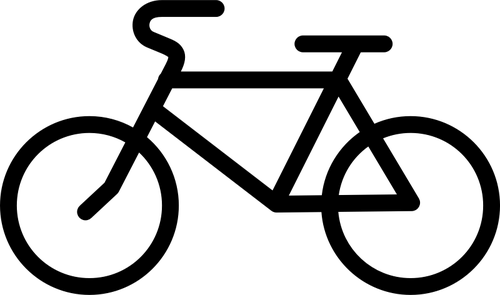
\includegraphics[width=.1\textwidth]{../bicycle.png}};

\draw[->, arrows={Triangle-Triangle}] (bs) -- (cl);
\node at (-0.4,2.75){PC} ;

\draw[->, arrows={-Triangle}, draw=red, transform canvas={xshift = 0.05cm}] (bs) -- (n1);
\draw[->, arrows={-Triangle}, draw=green, transform canvas={xshift = -0.05cm}] (n1) -- (bs);

\draw[->, arrows={-Triangle}, draw=red, transform canvas={xshift = 0.05cm}] (n1) -- (n3);
\draw[->, arrows={-Triangle}, draw=green, transform canvas={xshift = -0.05cm}] (n3) -- (n1);

\draw[->, arrows={-Triangle}, draw=red, transform canvas={yshift = 0.05cm}] (n1) -- (n2);
\draw[->, arrows={-Triangle}, draw=green, transform canvas={yshift = -0.05cm}] (n2) -- (n1);

\draw[->, arrows={-Triangle}, draw=red, transform canvas={xshift = 0.05cm}] (n2) -- (n4);
\draw[->, arrows={-Triangle}, draw=green, transform canvas={xshift = -0.05cm}] (n4) -- (n2);

\draw[->, arrows={-Triangle}, draw=red, transform canvas={yshift = 0.05cm}] (n3) -- (n4);
\draw[->, arrows={-Triangle}, draw=green, transform canvas={yshift = -0.05cm}] (n4) -- (n3);

\draw[->, arrows={Triangle-}, draw=red, transform canvas={yshift = 0.05cm}] (n3) -- (-0.5,-3.75);
\draw[->, arrows={Triangle-}, draw=green, transform canvas={yshift = -0.05cm}] (-0.5,-3.75) -- (n3);

\filldraw[color=green] (3-1,2+0.5) rectangle (3.5-1,2.5+0.5);
\node at (4.375-1,2.25+0.5)  {Collection};
\filldraw[color=red] (3-1,1.5+0.5) rectangle (3.5-1,2.0+0.5);
\node at (4.7-1,1.75+0.5)  {Dissemination};
\filldraw[color=black] (3-1,1.0+0.5) rectangle (3.5-1,1.5+0.5);
\node at (4.85-1,1.25+0.5)  {SerialForwarder};


\end{tikzpicture}}
\end{document}
